\documentclass{utitcphd_overleaf}
%% This file has version 0.98

%% MY CUSTOM SETTINGS

% \usepackage{caption}

% % Caption setup
% \captionsetup{
%   justification=centering,
%   font=normalfont
% }

\usepackage{listings}
\usepackage{xcolor}

% Setup for listings to handle JavaScript and JSX (as part of React)
\lstdefinelanguage{JavaScript}{
  keywords={const, let, function, if, else, return, class, export, default, extends},
  morecomment=[l]{//},
  morecomment=[s]{/*}{*/},
  morestring=[b]',
  morestring=[b]"
}

\lstdefinelanguage{json}{
    basicstyle=\normalfont\ttfamily,
    numbers=left,
    numberstyle=\scriptsize,
    stepnumber=1,
    numbersep=8pt,
    showstringspaces=false,
    breaklines=true,
    frame=lines,
    string=[s]{"}{"},
    stringstyle=\color{blue},
    comment=[l]{:},
    commentstyle=\color{black},
    morestring=[b]",
    morecomment=[l]{//},
    morecomment=[s]{/*}{*/},
    morekeywords={true,false,null}
}


\lstset{
  language=JavaScript,
  backgroundcolor=\color{white},   % choose the background color
  extendedchars=true,
  basicstyle=\footnotesize\ttfamily, % the size of the fonts that are used for the code
  showstringspaces=false,           % underline spaces within strings only
  showspaces=false,                 % show spaces everywhere with underscores; overrides 'showstringspaces'
  numbers=left,                     % where to put the line-numbers; possible values are (none, left, right)
  numberstyle=\tiny\color{gray},    % style used for line-numbers
  stepnumber=1,                     % step between two line-numbers. If it's 1, each line will be numbered
  numbersep=5pt,                    % how far the line-numbers are from the code
  tabsize=2,                        % sets default tabsize to 2 spaces
  breaklines=true,                  % sets automatic line breaking
  breakatwhitespace=false,          % sets if automatic breaks should only happen at whitespace
  commentstyle=\color{gray},       % comment color
  keywordstyle=\color{blue},        % keyword color
  stringstyle=\color{red},          % string literal color
  escapeinside={\%*}{*)},           % if you want to add LaTeX within your code
  morekeywords={render, componentDidMount}  % add more keywords if you need them
}


%%%%%%%%%%%%%%%%%%%%%%%%%%%%%%%%%%%%%%%%
%% Various definitions that are NEEDED
% \newcommand{\fancyTitle}{Data Driven Risk Management For Fire Services: \\ Chimney Fire Prediction Application}
% \newcommand{\saneTitle}{Data Driven Risk Management For Fire Services: Chimney Fire Prediction Application}
\title{\texorpdfstring{Data Driven Risk Management For Fire Services\\ ---\\Chimney Fire Prediction Application}{Data Driven Risk Management For Fire Services - Chimney Fire Prediction Application}}
% \title{\texorpdfstring{\fancyTitle}{\saneTitle}}
%% In the title, separate lines with "\\" and use " --- " instead of periods or semicolons (if any)

\author{Ömer Esas}                                         %% Provide author name, format "First von Last"

\SetPromoter{prof.~dr.~P. XXXXXXX}{University of Twente}
\SetSecondPromoter{prof.~dr.~S. XXXXXXX}{University of Twente}   %% Leave name empty or provide name
\SetAssistantPromoter{dr.~A. S. XXXXXXX}{University of Twente}     %% Leave name empty or provide name
\SetCoverDesigner{}                                                 %% Leave name empty or provide name
\SetDissertationNumber{XXX}                                         %% Provide number, format "xxx"
\SetDefenceDate{XXXXX, XXXXXXX 29, XXXXX}                           %% Provide date, format "DayInWeek, Month DayNumber, Year"
\SetDefenceTime{12.00}                                              %% Provide time, format "xx.xx"
\SetUTRector{prof.~dr.~ir.~A. Veldkamp}                                                      %% Leave empty (for Brinksma) or provide name
\SetBirthDate{December 15, 1993}                                       %% Provide date, format "Month xx, 2xxx"
\SetBirthPlace{Izmir, Turkey}                                 %% Provide city, format "city, country"
\SetISBN{xxx--xx--xxx--xxxx--x}                                     %% Provide true number, with format
                                                                    %%   "xxx--xx--xxx--xxxx--x", do not leave empty
\SetISSN{xxxx--xxxx, No. xx--xxx}                                   %% Some theses are in a journal series,
                                                                    %%   format "xxxx--xxxx, No. xx--xxx", or leave empty
\SetDOI{http://dx.doi.org/10.3990//x.xxxxxxxxxxxxx}                 %% Leave empty or provide DOI (digital object identifier),
                                                                    %%   format "http://dx.doi.org/10.3990//x.xxxxxxxxxxxxx"
\SetPrintShop{ITC Printing Department}  %% Privide name of printing agency, format "agency, city, country"
\SetFunnyStuff{}                                                    %% Leave empty ... or allow for additional logos, institutes, thesis
                                                                    %%   series, whatnots, et cetera.  This will be typeset mid-way on the
                                                                    %%   first left-hand page, below the dissertation committee.

%%%%%%%%%%%%%%%%%%%%%%%%%%%%%%%%%%%%%%%%

\begin{document}
%%%%%%%%%%%%%%%%%%%%%%%%%%%%%%%%%%%%%%%%%%%%%%%%%%%%%%%%%%%%%%
%% READ THIS CAREFULLY!!
%% This file version is 0.98; it works with same version of utitcphd.cls
%%
%% This file must be included through \include{thesis_frontpages}
%% from your main thesis tex file.
%% Do not change the contents of this file, EXCEPT for those
%% sections indicated as EDIT ZONE.  Typically in those zones
%% you MUST add your specifics for the thesis.
%% Search for "EDIT ZONE" in the file below, and again, only
%% do edits within those zones!
%%%%%%%%%%%%%%%%%%%%%%%%%%%%%%%%%%%%%%%%%%%%%%%%%%%%%%%%%%%%%%

\makeatletter
\hypersetup{pdfborder=0 0 0,pdftitle={\thetitle},pdfauthor={\theauthor}}
% \hypersetup{pdfborder=0 0 0,pdftitle={\texorpdfstring{\fancyTitle}{\saneTitle}},pdfauthor={\theauthor}}
%%%%%%%%%%%%%%%%%%%%%%%%%%%%%%%%%%%%%%%%%%%%%%%%%%%%%%%%%%%%%%
%% FIRST TITLE PAGE
%%%%%%%%%%%%%%%%%%%%%%%%%%%%%%%%%%%%%%%%%%%%%%%%%%%%%%%%%%%%%%
\pagenumbering{alph}

\thispagestyle{empty}
{\Huge
\begin{center}

\textbf{\thetitle}\\[18mm]

\theauthor
\end{center}
}
\clearpage

%%%%%%%%%%%%%%%%%%%%%%%%%%%%%%%%%%%%%%%%%%%%%%%%%%%%%%%%%%%%%%
%% TITLE BACKPAGE
%%%%%%%%%%%%%%%%%%%%%%%%%%%%%%%%%%%%%%%%%%%%%%%%%%%%%%%%%%%%%%

\thispagestyle{empty}

\cleardoublepage

%%%%%%%%%%%%%%%%%%%%%%%%%%%%%%%%%%%%%%%%%%%%%%%%%%%%%%%%%%%%%%
%% OFFICIAL PAGE
%%%%%%%%%%%%%%%%%%%%%%%%%%%%%%%%%%%%%%%%%%%%%%%%%%%%%%%%%%%%%%
\thispagestyle{empty}
{\LARGE
	\begin{center}
		
		\textbf{\MakeUppercase{\thetitle}}
		
		\vfill
		
		\so{EngD Thesis}
		
		\vfill
		
		{\Large to obtain the degree of\\
            Engineering Doctorate (EngD) at the University of Twente,\\
			on the authority of the rector magnificus,\\
			\@UTRector,\\
			on account of the decision of the Doctorate Board,\\
			to be defended\\
			on \@DefenceDate\ at \@DefenceTime\\}
		
		\vfill
		
		{\Large by}
		
		\vfill
		
		{\textbf{\theauthor}\\
			born on \@BirthDate\\
			in \@PlaceofBirth}
	\end{center}
}
\clearpage

%%%%%%%%%%%%%%%%%%%%%%%%%%%%%%%%%%%%%%%%%%%%%%%%%%%%%%%%%%%%%%
%% APPRVOVAL AND (C) PAGE
%%%%%%%%%%%%%%%%%%%%%%%%%%%%%%%%%%%%%%%%%%%%%%%%%%%%%%%%%%%%%%
\thispagestyle{empty}
\noindent This EngD Thesis has been approved by: \\[\baselineskip]

\noindent\@Promoter\ (promoter)\\
\ifsecondpromoter\noindent\@SecondPromoter\ (promoter) \\ \fi
\ifassistantpromoter\noindent\@AssistantPromoter\ (assistant promoter) \\ \fi
\ifsecondassistantpromoter\noindent\@SecondAssistantPromoter\ (assistant promoter) \fi

\vfill

\iffunnystuff \@FunnyStuff \fi    %% Allow for additional logos, institutes, thesis series, whatnots, et cetera.

\vfill

% \noindent ITC dissertation number \@DissertationNumber \\
% ITC, P.O. Box 217, 7500 AE Enschede, The Netherlands

{\small\vspace*{2mm}

% \begin{tabbing}
% Printed byby \= \kill
% ISBN:                    \> \@ISBN \\
% \ifissn ISSN:            \> \@ISSN \\ \fi
% \ifdoi DOI:              \> \@DOI  \\ \fi
% \ifprintshop Printed by: \> \@PrintShop \\ \fi
% \end{tabbing}

\vspace*{-2mm}  % Is 2mm minus the extra tabbing afterspace

\noindent\copyright\ \theauthor, Enschede, The Netherlands\\
\ifcoverdesigner\copyright\ Cover design by \@CoverDesigner\\ \fi
All rights reserved. No part of this publication may be reproduced without the prior written
permission of the author.

\vspace*{2mm}
}

\noindent
\includegraphics[width=\textwidth]{support/UT_logo.pdf}

\clearpage

%%%%%%%%%%%%%%%%%%%%%%%%%%%%%%%%%%%%%%%%%%%%%%%%%%%%%%%%%%%%%%

\clearpage
%%%%%%%%%%%%%%%%%%%%%%%%%%%%%%%%%%%%%%%%%%%%%%%%%%%%%%%%%%%%%%
\makeatother


\openright
\frontmatter

%-------------------------------------------------------------------------------
% Preface
%-------------------------------------------------------------------------------
% \include{Abstract}
% \include{Samenvatting}
% \include{Acknowledgments} %% Remove for review
% \include{nomenclature}

%-------------------------------------------------------------------------------
% Index
%-------------------------------------------------------------------------------
\tableofcontents

%-------------------------------------------------------------------------------
% Main Matter
%-------------------------------------------------------------------------------
\mainmatter

\chapter{Introduction}
\label{chap:introduction}

Lorem ipsum dolor sit amet, consectetur adipiscing elit. Nullam congue sed lectus sed finibus. Suspendisse posuere dapibus erat, sed eleifend libero congue nec. Phasellus ut vehicula purus. Cras feugiat augue non interdum sodales. Sed luctus neque nec venenatis dictum. Donec porttitor, erat at dignissim tristique, arcu ipsum laoreet elit, ac vestibulum nibh turpis at nibh. Maecenas iaculis fermentum accumsan. In hac habitasse platea dictumst. Maecenas auctor tortor rutrum, consequat dolor ut, aliquam ligula.

Donec ac imperdiet ex, vel ultricies arcu. Vivamus molestie massa tincidunt, interdum lectus id, pellentesque lorem. Nam elementum tempus tortor ut ornare. In blandit hendrerit odio vitae aliquam. Phasellus fringilla a ante sed varius. Sed sit amet vulputate metus. Mauris at quam nibh.

Proin ac ex cursus ipsum elementum fermentum. Pellentesque tristique, risus non lacinia volutpat, mi dolor interdum erat, sit amet tincidunt ante sapien quis odio. Donec mollis hendrerit magna vel varius. Aenean et nulla sit amet orci finibus imperdiet. Etiam non erat eu ligula consectetur facilisis. Curabitur et pulvinar nisi. Quisque fermentum ac erat et hendrerit. Integer ullamcorper ut orci a elementum. Nulla nec dapibus metus. Proin ut lectus non ipsum lobortis viverra.

Nunc vel mauris eu eros finibus faucibus id sit amet dui. Aenean a sollicitudin diam. Donec sollicitudin ultricies purus, semper tempus lectus egestas vel. Ut vel volutpat odio, eget suscipit dui. Sed rutrum euismod fringilla. Nulla convallis, elit quis convallis dictum, diam tellus fringilla neque, vel fringilla felis tortor non leo. Nunc augue est, posuere a arcu sed, convallis imperdiet tellus.

Fusce placerat at sem nec congue. Vestibulum ultricies neque sed sapien convallis, non ultrices mi ultricies. Morbi ultrices risus sit amet enim mattis pharetra nec sit amet dolor. Duis euismod, est ut rhoncus rutrum, lacus dui auctor enim, sit amet ullamcorper purus neque efficitur diam. Fusce scelerisque et justo convallis viverra. Curabitur id malesuada nibh, non dignissim erat. Donec consequat id augue ac tempus. Duis in posuere purus. Vivamus iaculis vestibulum ipsum ac tempor. Proin et tincidunt sapien, ut tincidunt sapien. Morbi in eleifend nulla, at rutrum lorem. Integer congue nibh et vehicula cursus. Praesent a sem erat.

\section{Background}

Lorem ipsum dolor sit amet, consectetur adipiscing elit. Nullam congue sed lectus sed finibus. Suspendisse posuere dapibus erat, sed eleifend libero congue nec. Phasellus ut vehicula purus. Cras feugiat augue non interdum sodales. Sed luctus neque nec venenatis dictum. Donec porttitor, erat at dignissim tristique, arcu ipsum laoreet elit, ac vestibulum nibh turpis at nibh. Maecenas iaculis fermentum accumsan. In hac habitasse platea dictumst. As shown in Figure~\ref{fig:yourlabel}, ...

\begin{figure}[ht]
  \centering
  
\includegraphics[width=0.8\textwidth]{my_images/kitten.jpeg}
  \caption{Your caption text goes here}
  \label{fig:yourlabel}
\end{figure}


Donec ac imperdiet ex, vel ultricies arcu. Vivamus molestie massa tincidunt, interdum lectus id, pellentesque lorem. Nam elementum tempus tortor ut ornare. In blandit hendrerit odio vitae aliquam. Phasellus fringilla a ante sed varius. Sed sit amet vulputate metus. Mauris at quam nibh.

Proin ac ex cursus ipsum elementum fermentum. Pellentesque tristique, risus non lacinia volutpat, mi dolor interdum erat, sit amet tincidunt ante sapien quis odio. Donec mollis hendrerit magna vel varius. Aenean et nulla sit amet orci finibus imperdiet. Etiam non erat eu ligula consectetur facilisis. Curabitur et pulvinar nisi. Quisque fermentum ac erat et hendrerit. Integer ullamcorper ut orci a elementum. Nulla nec dapibus metus. Proin ut lectus non ipsum lobortis viverra.

Nunc vel mauris eu eros finibus faucibus id sit amet dui. Aenean a sollicitudin diam. Donec sollicitudin ultricies purus, semper tempus lectus egestas vel. Ut vel volutpat odio, eget suscipit dui. Sed rutrum euismod fringilla. Nulla convallis, elit quis convallis dictum, diam tellus fringilla neque, vel fringilla felis tortor non leo. Nunc augue est, posuere a arcu sed, convallis imperdiet tellus.

Fusce placerat at sem nec congue. Vestibulum ultricies neque sed sapien convallis, non ultrices mi ultricies. Morbi ultrices risus sit amet enim mattis pharetra nec sit amet dolor. Duis euismod, est ut rhoncus rutrum, lacus dui auctor enim, sit amet ullamcorper purus neque efficitur diam. Fusce scelerisque et justo convallis viverra. Curabitur id malesuada nibh, non dignissim erat. Donec consequat id augue ac tempus. Duis in posuere purus. Vivamus iaculis vestibulum ipsum ac tempor. Proin et tincidunt sapien, ut tincidunt sapien. Morbi in eleifend nulla, at rutrum lorem. Integer congue nibh et vehicula cursus. Praesent a sem erat.

\section{Motivation}

Lorem ipsum dolor sit amet, consectetur adipiscing elit. Nullam congue sed lectus sed finibus. Suspendisse posuere dapibus erat, sed eleifend libero congue nec. Phasellus ut vehicula purus. Cras feugiat augue non interdum sodales. Sed luctus neque nec venenatis dictum. Donec porttitor, erat at dignissim tristique, arcu ipsum laoreet elit, ac vestibulum nibh turpis at nibh. Maecenas iaculis fermentum accumsan. In hac habitasse platea dictumst.

\section{Organization}

Lorem ipsum dolor sit amet, consectetur adipiscing elit. Nullam congue sed lectus sed finibus. Suspendisse posuere dapibus erat, sed eleifend libero congue nec. Phasellus ut vehicula purus. Cras feugiat augue non interdum sodales. Sed luctus neque nec venenatis dictum. Donec porttitor, erat at dignissim tristique, arcu ipsum laoreet elit, ac vestibulum nibh turpis at nibh. Maecenas iaculis fermentum accumsan. In hac habitasse platea dictumst.

\section{Outline of the EngD Thesis}

Lorem ipsum dolor sit amet, consectetur adipiscing elit. Nullam congue sed lectus sed finibus. Suspendisse posuere dapibus erat, sed eleifend libero congue nec. Phasellus ut vehicula purus. Cras feugiat augue non interdum sodales. Sed luctus neque nec venenatis dictum. Donec porttitor, erat at dignissim tristique, arcu ipsum laoreet elit, ac vestibulum nibh turpis at nibh. Maecenas iaculis fermentum accumsan. In hac habitasse platea dictumst.

\chapter{Problem Investigation}
\label{chap:problem}

\section{Mathematical Model Analysis}
\section{IT Systems of Twente Fire Services}

Lorem ipsum dolor sit amet, consectetur adipiscing elit. Nullam congue sed lectus sed finibus. Suspendisse posuere dapibus erat, sed eleifend libero congue nec. Phasellus ut vehicula purus. Cras feugiat augue non interdum sodales. Sed luctus neque nec venenatis dictum. Donec porttitor, erat at dignissim tristique, arcu ipsum laoreet elit, ac vestibulum nibh turpis at nibh. Maecenas iaculis fermentum accumsan. In hac habitasse platea dictumst. Maecenas auctor tortor rutrum, consequat dolor ut, aliquam ligula.

\chapter{Methodology}
\label{chap:management}

Lorem ipsum dolor sit amet, consectetur adipiscing elit. Nullam congue sed lectus sed finibus. Suspendisse posuere dapibus erat, sed eleifend libero congue nec. Phasellus ut vehicula purus. Cras feugiat augue non interdum sodales. Sed luctus neque nec venenatis dictum. Donec porttitor, erat at dignissim tristique, arcu ipsum laoreet elit, ac vestibulum nibh turpis at nibh. Maecenas iaculis fermentum accumsan. In hac habitasse platea dictumst. Maecenas auctor tortor rutrum, consequat dolor ut, aliquam ligula.

\section{Design Approach}

Mention why agile, use node.js and docker

\section{Architectural Design of Milestones}

\subsection{Milestone 1}

In the design phase of Milestone 1, our goal was to quickly establish a functioning software tool that relied on historical data for its predictions. By the conclusion of this milestone, we aimed to have a backend API capable of forecasting chimney fire risks across various areas of Twente region using past weather data. Even though employing historical data compromises the accuracy of our predictions, it simplifies implementation and allows us to quickly integrate and test the IT systems, ensuring all components operate smoothly and validate the system's overall functionality from the outset. This ensures all components are able to function as expected right from the start and establishes a reliable basis for the features planned in subsequent milestones. With this mindset, we designed the architecture of Milestone 1 to consist of a simple API and the necessary IT systems from Twente Fire Brigade for visualization purposes, as seen in Figure~\ref{fig:iteration_1_arch}.

\begin{figure}[ht]
  \centering
  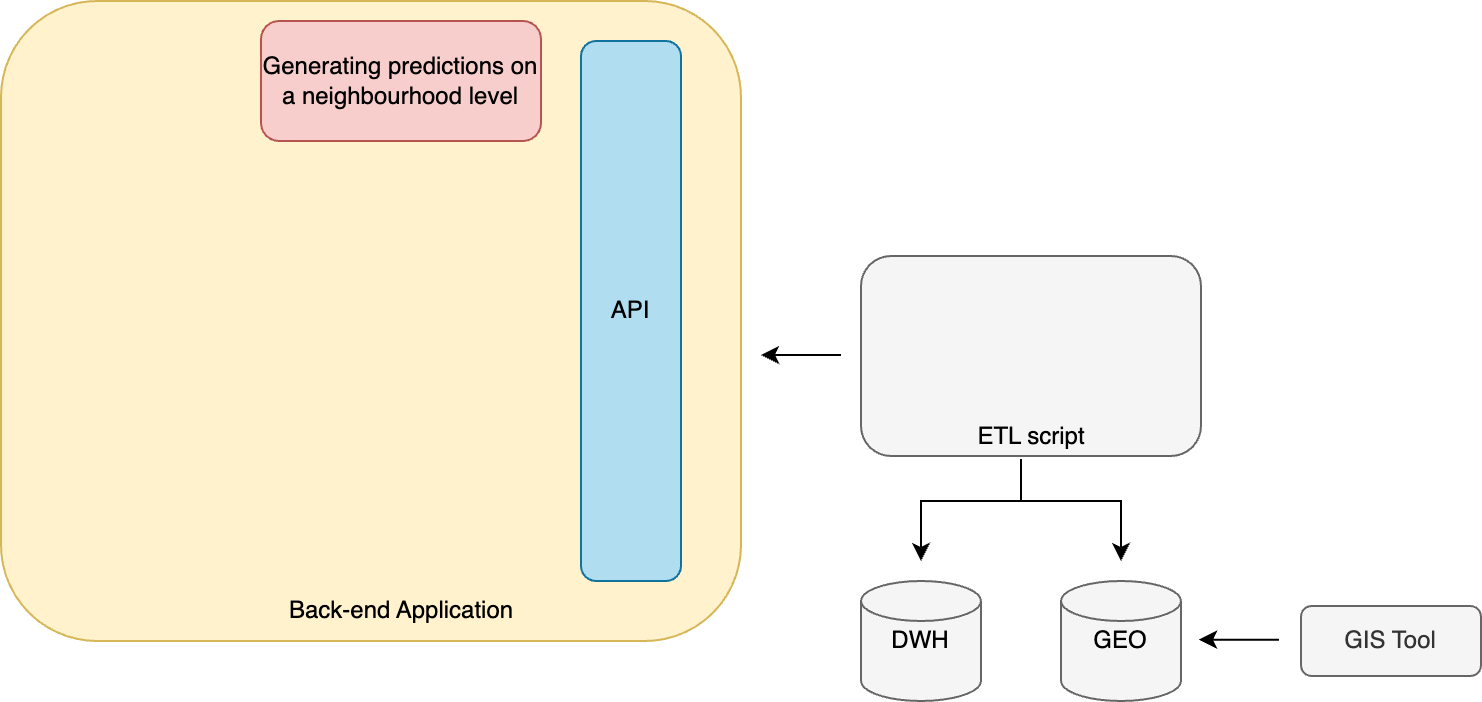
\includegraphics[width=1\textwidth]{my_images/milestones/iteration_1_arch.png}
  \caption{Architectural Diagram of Milestone 1}
  \label{fig:iteration_1_arch}
\end{figure}

The backend API is designed to serve as a source for generating predictions based on historical data. To carry out data fetching and saving, Twente Fire Brigade is to develop an Extract-Transform-Load (ETL) script that makes HTTP GET requests to the API. To display the predictions on an interactive map, a Geo-Information-System (GIS) tool, which is already utilised for visualization tasks at Twente Fire Brigade as can be seen in Figure~\ref{fig:iteration_1_gis}, can be connected to the data warehouse or geo-database of Twente Fire Brigade and get and display the predictions that are saved those databases. Last but not least, to realise this and subsequent architectures, the application is to be deployed Azure cloud platform in a Docker container, using the Azure account of Twente Fire Brigade.

\begin{figure}[ht]
  \centering
  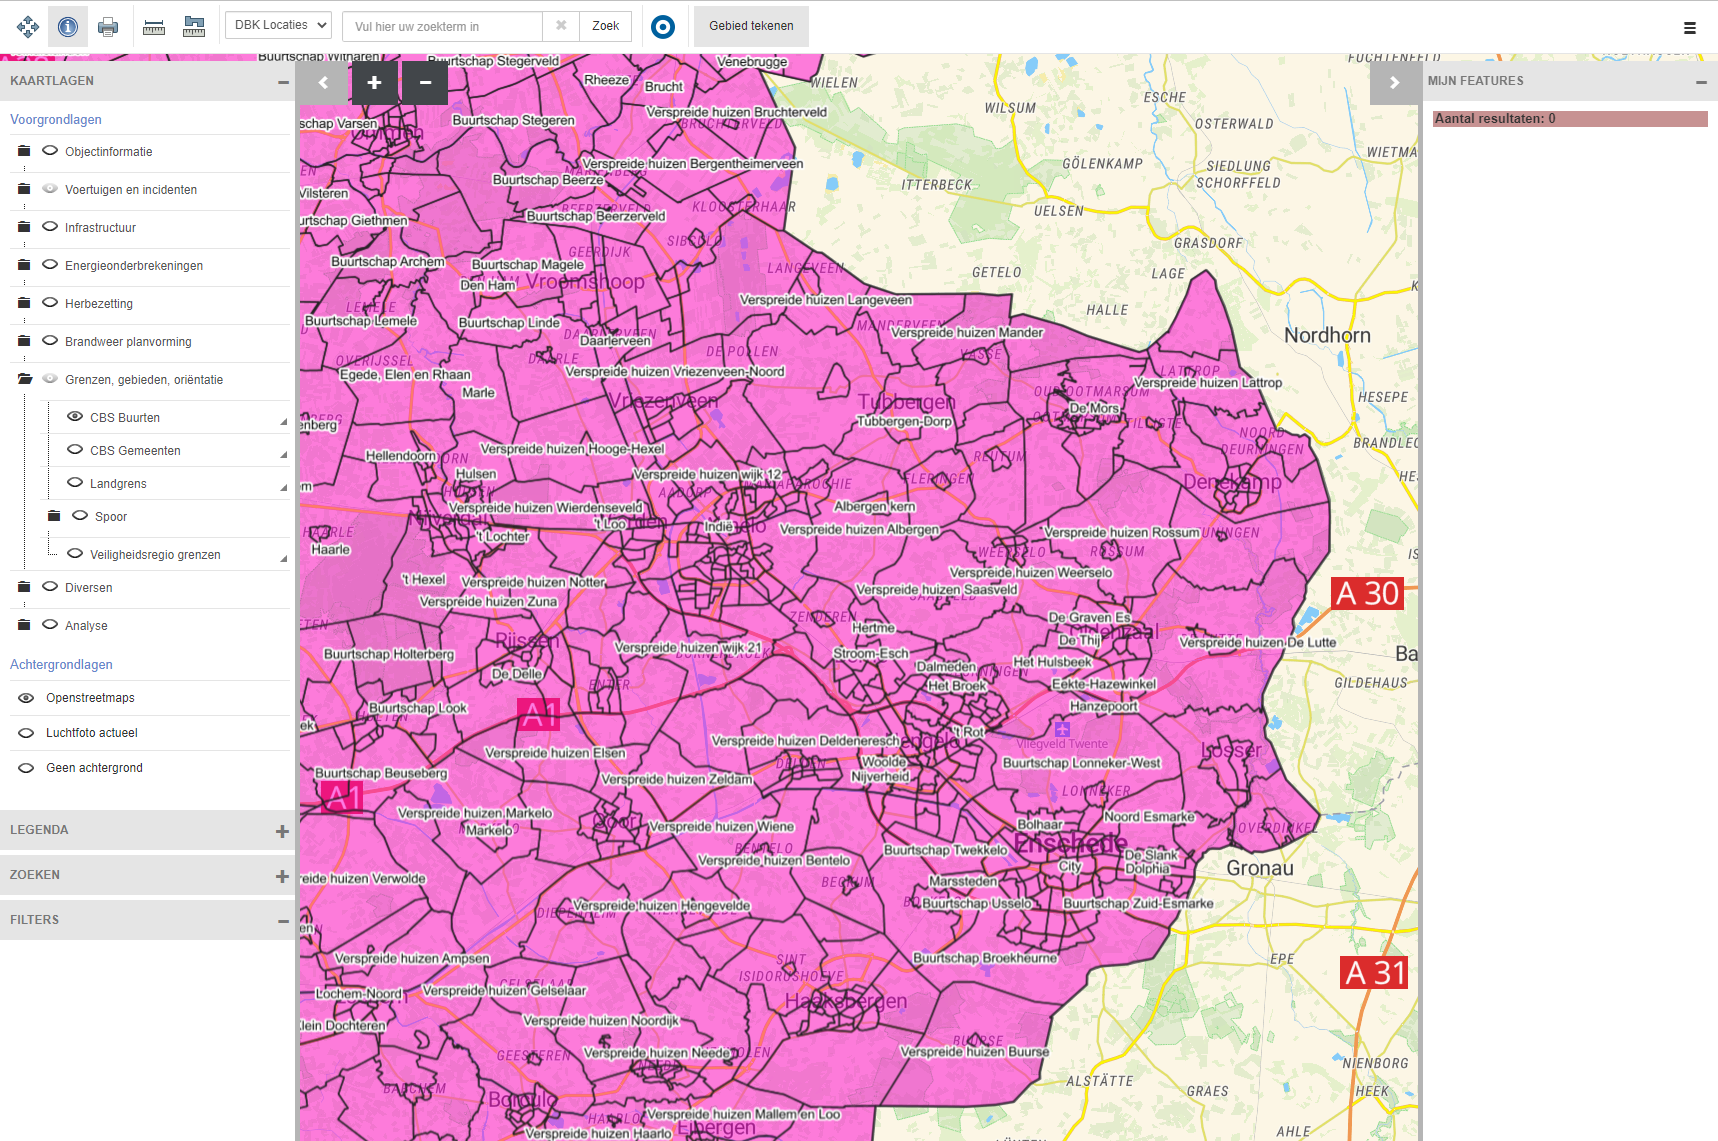
\includegraphics[width=1\textwidth]{my_images/milestones/iteration_1_gis.png}
  \caption{Screenshot of the GIS tool at Twente Fire Brigade}
  \label{fig:iteration_1_gis}
\end{figure}

\subsection{Milestone 2}

Building upon the solid foundation established in Milestone 1, Milestone 2 of the chimney fire risk prediction application development significantly enhances both the depth and the reliability of our predictions. In this iteration, we have integrated the capability to receive and process real-time weather forecast data, which allows the backend application to generate more accurate and timely predictions about chimney fire risks in the Twente region, which can be seen in Figure~\ref{fig:iteration_2_arch}.

\begin{figure}[ht]
  \centering
  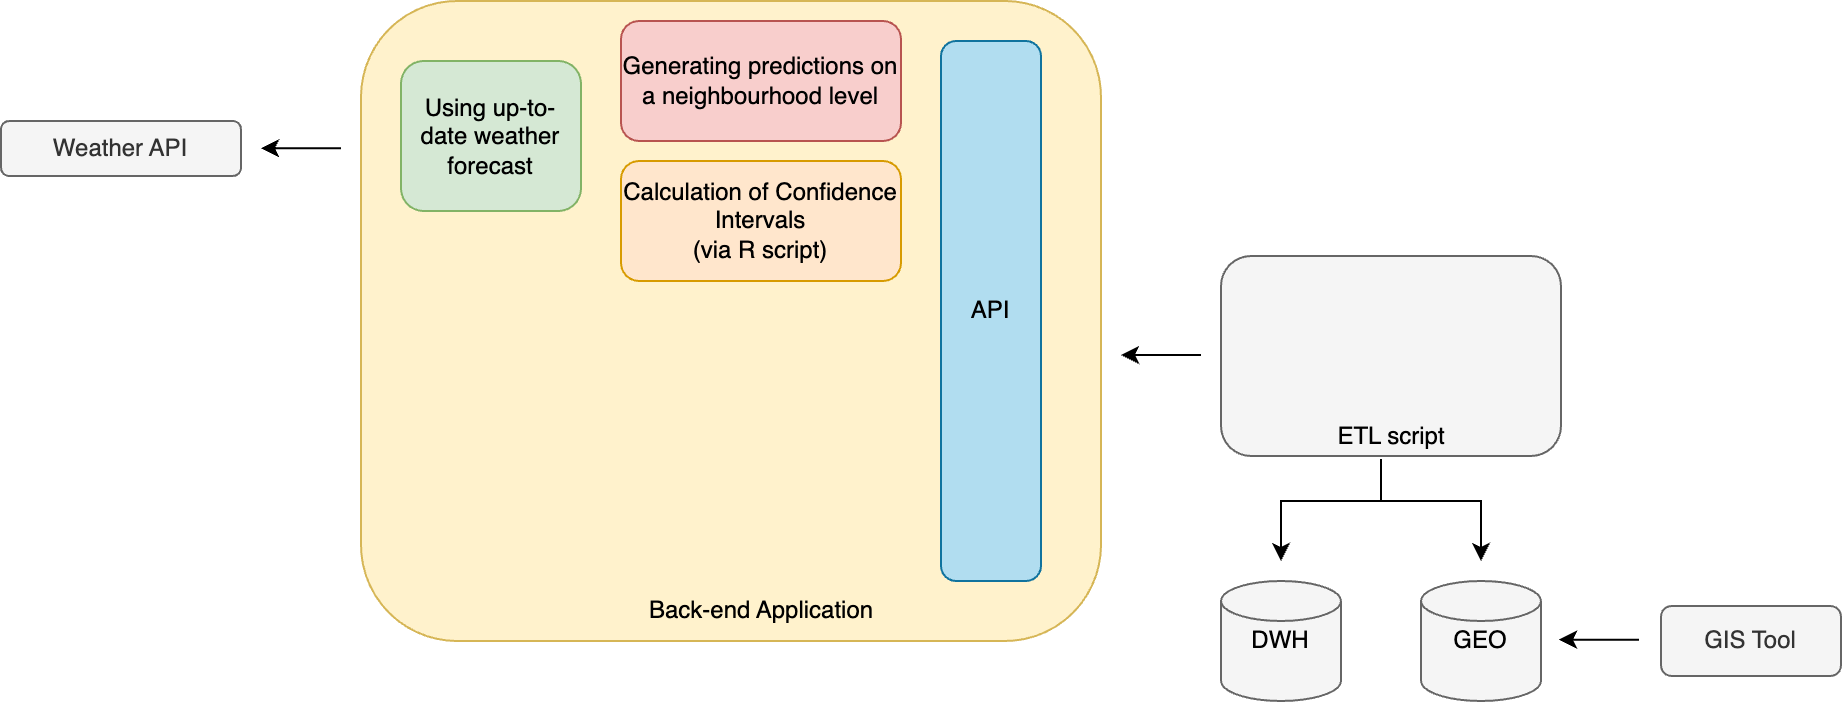
\includegraphics[width=1\textwidth]{my_images/milestones/iteration_2_arch.png}
  \caption{Architectural Diagram of Milestone 2}
  \label{fig:iteration_2_arch}
\end{figure}

Specifically, the backend API now connects to an external weather forecasting service to obtain up-to-date weather predictions. These predictions include critical weather parameters that significantly influence chimney fire occurrences, such as air temperature, wind speed and wind chill. By incorporating current weather data, the API can adjust its risk assessments on a daily basis to reflect changing environmental conditions, thereby providing predictions that are not only based on historical weather patterns but also on the present weather scenario.

Another significant enhancement in Milestone 2 is the introduction of confidence intervals in the prediction outputs. Confidence intervals provide a statistical range that is likely to contain the true value of the number of chimney fires expected, offering an additional layer of information about the reliability and precision of the predictions. This calculation of confidence intervals might require the use of spatial statistics libraries in R, necessitating the running of some R processes in the backend application to handle these computations effectively. This feature is particularly valuable as it helps decision-makers at the Twente Fire Brigade understand the uncertainty associated with the predictions, aiding them in risk assessment and resource allocation more effectively.

In short, Milestone 2 marks a significant step forward in our project, moving from a prototype that provided basic predictions based on historical data to a sophisticated tool that utilizes real-time data to enhance prediction accuracy and utility.

\subsection{Milestone 3}

Lorem ipsum dolor sit amet, consectetur adipiscing elit. Nullam congue sed lectus sed finibus. Suspendisse posuere dapibus erat, sed eleifend libero congue nec. Phasellus ut vehicula purus. Cras feugiat augue non interdum sodales. Sed luctus neque nec venenatis dictum. Donec porttitor, erat at dignissim tristique, arcu ipsum laoreet elit, ac vestibulum nibh turpis at nibh. Maecenas iaculis fermentum accumsan. In hac habitasse platea dictumst.

\subsection{Milestone 4}

Lorem ipsum dolor sit amet, consectetur adipiscing elit. Nullam congue sed lectus sed finibus. Suspendisse posuere dapibus erat, sed eleifend libero congue nec. Phasellus ut vehicula purus. Cras feugiat augue non interdum sodales. Sed luctus neque nec venenatis dictum. Donec porttitor, erat at dignissim tristique, arcu ipsum laoreet elit, ac vestibulum nibh turpis at nibh. Maecenas iaculis fermentum accumsan. In hac habitasse platea dictumst.

\chapter{Implementation}
\label{chap:implementation}

Lorem ipsum dolor sit amet, consectetur adipiscing elit. Nullam congue sed lectus sed finibus. Suspendisse posuere dapibus erat, sed eleifend libero congue nec. Phasellus ut vehicula purus. Cras feugiat augue non interdum sodales. Sed luctus neque nec venenatis dictum. Donec porttitor, erat at dignissim tristique, arcu ipsum laoreet elit, ac vestibulum nibh turpis at nibh. Maecenas iaculis fermentum accumsan. In hac habitasse platea dictumst. Maecenas auctor tortor rutrum, consequat dolor ut, aliquam ligula.

% \begin{lstlisting}[label={lst:listing-js}, language=JavaScript, caption=React Component Example]
% import React, { Component } from 'react';

% class App extends Component {
%   componentDidMount() {
%       // Code to run on component mount
%   }

%   render() {
%     return (
%       <div>
%         Hello, world!
%       </div>
%     );
%   }
% }

% export default App;
% \end{lstlisting}

% An example table can be seen in Listing \ref{lst:listing-js}.


\section{Implementation of Milestones}

\subsection{Milestone 1}

As the first in the implementation phase, to start producing the predictions, the application logic implemented is illustrated in Figure~\ref{fig:m1_logic}, where the application model elements from Archimate modeling language are utilized. The application first receives an API request from an application of Twente Fire Brigade, which can be a Geo-Information System (GIS) tool or an Extract- Transform-Load (ETL) script. The application then validates if the input parameters are valid, in other words, if the date is a date string in proper format and if the area code is a valid CBS area code, such as “GM0153” for the city of “Enschede” or “WK015303” for the district of “Twekkelerveld” in Enschede. If both input parameters are valid, then the application calculates the predicted number of chimney fires for that area on that day.

\begin{figure}[ht]
  \centering
  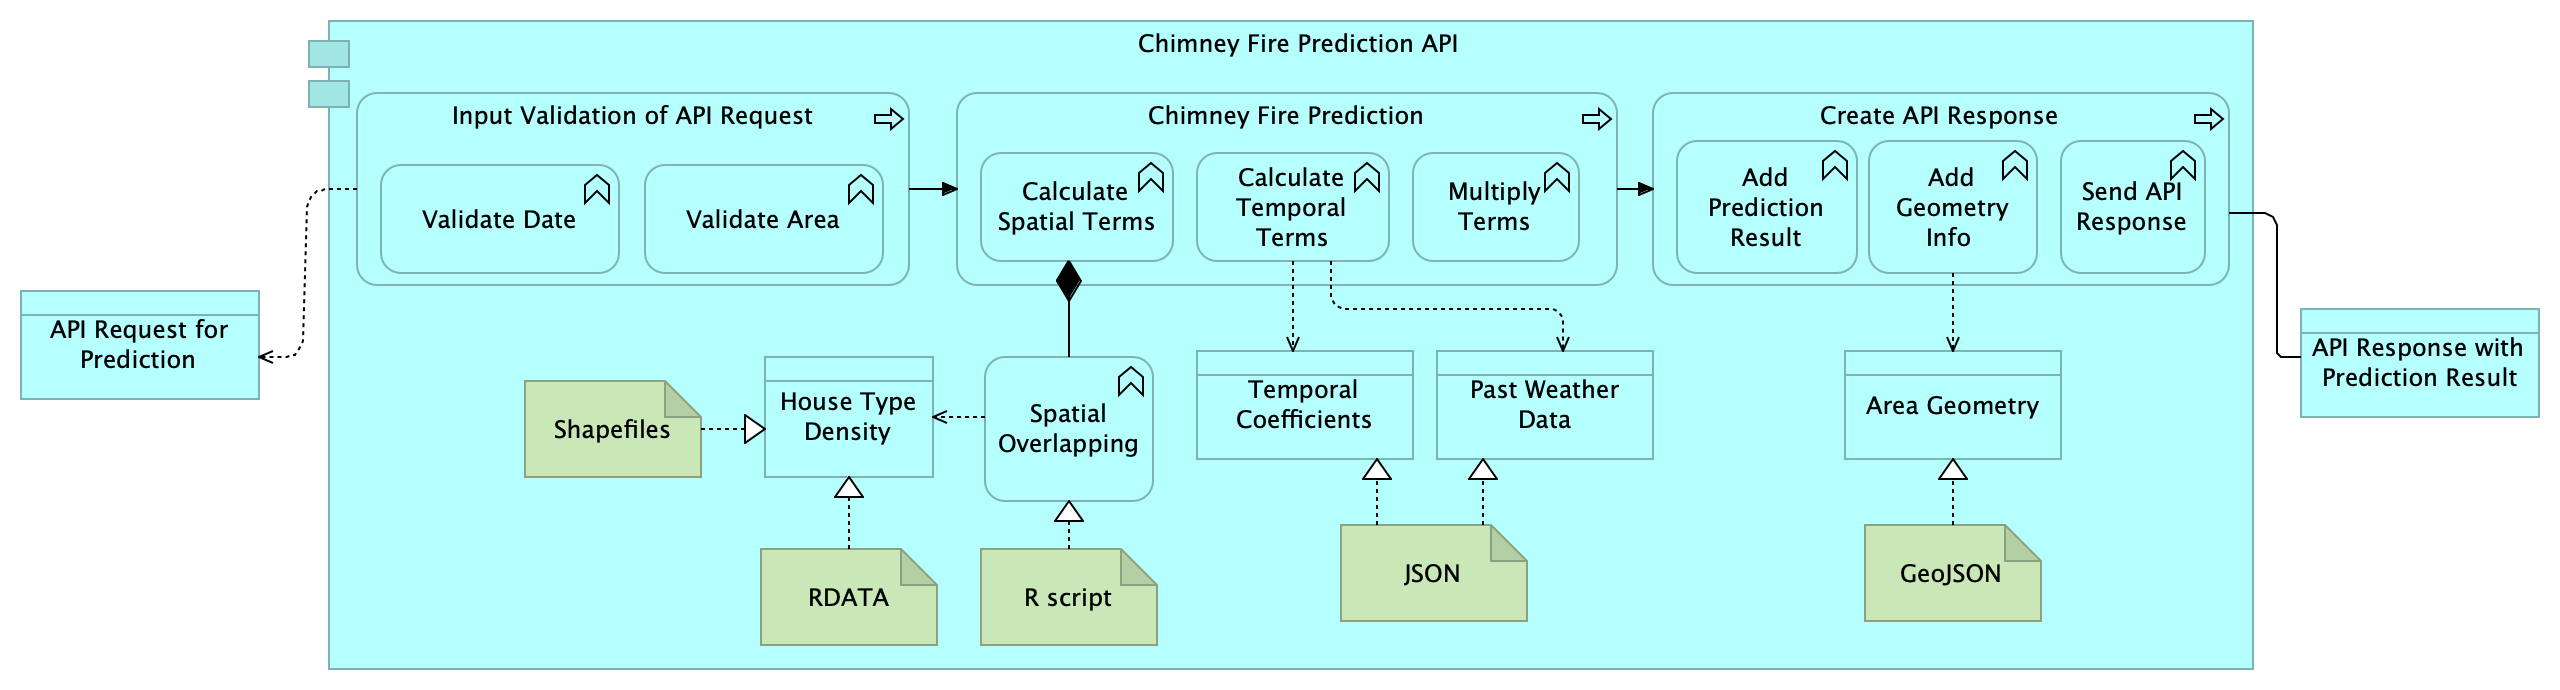
\includegraphics[width=1\textwidth]{my_images/milestones/m1.png}
  \caption{Application Logic of Milestone 1}
  \label{fig:m1_logic}
\end{figure}

To avoid complexity in the first milestone, we decided to simplify the prediction generation process, which consists of calculating spatial and temporal terms and multiplying them to have the actual prediction result. To have the spatial terms, we took a straightforward approach and implemented this in a similar way to the code used in the research paper of this project. More specifically, we used the density information of houses of different types in the format of “shapefile” and “.RData” objects. Then, we made use of the “spatial overlapping” functions in R to have the spatial terms for the area given as input parameter. As for the temporal terms for that date, we utilised only the historical weather data, namely, the wind speed and wind chill values for the Twente region in 2020, which we stored as JSON files alongside the temporal coefficients used to calculate the temporal terms for the date given as input parameter in the API request. Multiplying the calculated spatial terms for the area of interest and temporal terms for the date of interest, we have the predicted number of chimney fires for that area on that date.

The course of the API request ends with creating and sending the API response in JSON format. Finally, the geometry information of the area is included in the response, in case the API request is made by the GIS tool of the Twente Fire Brigade, which needs this geometry information in GeoJSON format so that it is able to draw the borders of the area of interest on the map of the Twente. In short, at the end of Milestone 1, we implemented prototype which can process API requests and respond with a prediction result, although only using historical weather data instead of up-to- date weather forecast, hence not responding with the most accurate predictions.

\subsection{Milestone 2}
\subsection{Milestone 3}
\subsection{Milestone 4}

\section{Frontend Application}

Lorem ipsum dolor sit amet, consectetur adipiscing elit. Nullam congue sed lectus sed finibus. Suspendisse posuere dapibus erat, sed eleifend libero congue nec. Phasellus ut vehicula purus. Cras feugiat augue non interdum sodales. Sed luctus neque nec venenatis dictum. Donec porttitor, erat at dignissim tristique, arcu ipsum laoreet elit, ac vestibulum nibh turpis at nibh. Maecenas iaculis fermentum accumsan. In hac habitasse platea dictumst. Maecenas auctor tortor rutrum, consequat dolor ut, aliquam ligula.

\chapter{Deployment \& Validation}
\label{chap:deployment}

\section{Deployment}

\section{Validation}


\chapter{Conclusion and Future Work}
\label{chap:conclusion}

%-------------------------------------------------------------------------------
% Appendix
%-------------------------------------------------------------------------------
\appendix
\chapter{GitHub Repository}
\label{app:additionaldata}

Here you can include additional data relevant to your thesis. This appendix is now formatted as an appendix section.

\chapter{API Endpoints}
\label{app:additionaldata}

Here you can include additional data relevant to your thesis. This appendix is now formatted as an appendix section.

\chapter{Example API Responses}
\label{app:additionaldata}

\begin{lstlisting}[language=json, caption=Example API Response]
{
    "lastWeatherFetchTimestamp": "17-04-2024 15:15:13",
    "predictions": {
        "areaId": "GM0153",
        "prediction": [
            {
                "date": "17-04-2024",
                "numberOfFires": "0.064677",
                "lowerBoundOfFires": "0.061271",
                "upperBoundOfFires": "0.068083"
            },
            {
                "date": "18-04-2024",
                "numberOfFires": "0.063505",
                "lowerBoundOfFires": "0.060078",
                "upperBoundOfFires": "0.066931"
            },
            {
                "date": "19-04-2024",
                "numberOfFires": "0.069518",
                "lowerBoundOfFires": "0.065613",
                "upperBoundOfFires": "0.073422"
            },
            {
                "date": "20-04-2024",
                "numberOfFires": "0.081339",
                "lowerBoundOfFires": "0.076496",
                "upperBoundOfFires": "0.086181"
            },
            {
                "date": "21-04-2024",
                "numberOfFires": "0.074268",
                "lowerBoundOfFires": "0.069827",
                "upperBoundOfFires": "0.078709"
            },
            {
                "date": "22-04-2024",
                "numberOfFires": "0.086056",
                "lowerBoundOfFires": "0.080469",
                "upperBoundOfFires": "0.091644"
            },
            {
                "date": "23-04-2024",
                "numberOfFires": "0.071638",
                "lowerBoundOfFires": "0.067111",
                "upperBoundOfFires": "0.076164"
            },
            {
                "date": "24-04-2024",
                "numberOfFires": "0.058141",
                "lowerBoundOfFires": "0.054491",
                "upperBoundOfFires": "0.061790"
            },
            {
                "date": "25-04-2024",
                "numberOfFires": "0.057063",
                "lowerBoundOfFires": "0.053378",
                "upperBoundOfFires": "0.060747"
            },
            {
                "date": "26-04-2024",
                "numberOfFires": "0.067903",
                "lowerBoundOfFires": "0.063232",
                "upperBoundOfFires": "0.072574"
            },
            {
                "date": "27-04-2024",
                "numberOfFires": "0.097660",
                "lowerBoundOfFires": "0.086680",
                "upperBoundOfFires": "0.108641"
            }
        ]
    }
}
\end{lstlisting}

\chapter{Screenshots of the Frontend Application}
\label{app:additionaldata}



\listoffigures
\listoftables

%-------------------------------------------------------------------------------
% Bibliography
%-------------------------------------------------------------------------------
\bibliographystyle{abbrv}
\bibliography{references}                   %% The name of your bib file

%-------------------------------------------------------------------------------
% Miscellaneous
%-------------------------------------------------------------------------------
\include{misc}  

\end{document}
